\documentclass[11pt]{article}
\usepackage{graphicx}
\usepackage[margin=2.5cm]{geometry}
\usepackage{tikz}
\usepackage{indentfirst}
\usepackage{tabularx}
\usepackage{listingsutf8}
\usepackage{color}
\usepackage[portuguese]{babel}

\graphicspath{{./images/}}

\def\checkmark{\tikz\fill[scale=0.4](0,.35) -- (.25,0) -- (1,.7) -- (.25,.15) -- cycle;} 
\setlength{\parskip}{0.5em}

\lstset{
	belowcaptionskip=1\baselineskip,
	captionpos=b,
	frame=tb,
	language=C,
	aboveskip=3mm,
	belowskip=3mm,
	showstringspaces=false,
	columns=flexible,
	basicstyle={\small\ttfamily},
	numbers=none,
	numberstyle=\tiny\color{gray},
	keywordstyle=\color{blue},
	commentstyle=\color{dkgreen},
	stringstyle=\color{mauve},
	breaklines=true,
	breakatwhitespace=true,
	tabsize=3,
	inputencoding=utf8,
	extendedchars=true,
	literate={á}{{\'a}}1 {ã}{{\~a}}1 {à}{{\`a} }1 {Ã}{{\~A}}1 {ó}{{\'o}}1 {Ó}{{\'O}}1 {Í}{{\'I}}1 {í}{{\'i}}1 {é}{{\'e}}1 {ç}{{\c{c}}}1 {Ç}{{\c{C}}}1 {ú}{{\'u}}1
}

\begin{document}
	\begin{titlepage}
	\begin{center}
		
\includegraphics[width=0.6\textwidth]{logo-isec}
		
		\vspace*{\fill}
		
		\Huge
		\textbf{Conhecimento e Raciocínio}
		
		\LARGE
		2020 - 2021
		
		\vspace{1.5cm}
		
		\huge
		Redes Neuronais
		
		\LARGE
		Identificação de Caracteres Gregos
		
		\vspace{2.5cm}
		
		\textbf{Ângelo Paiva - 2019129023} \\
		\textbf{José Almeida - 2019129077}
		
		
		\vfill
		\vspace*{\fill}
		
		\normalsize
		Licenciatura de Engenharia Informática \\
		26 de junho de 2021		
	\end{center}
\end{titlepage}
	
	\tableofcontents
	\pagebreak
	
	\large
	\section{Introdução}
	
	\normalsize
	Este trabalho, feito no âmbito da Unidade Curricular de Conhecimento e Raciocínio, tem como objetivo o desenvolvimento e estudo estatístico de redes neuronais para identificação de alguns caracteres gregos. A linguagem e tecnologia usada para esse efeito é o MATLAB. Adicionalmente, o trabalho prático inclui uma aplicação gráfica que permite criar, treinar e simular redes.
	
	\large
	\section{Conversão e Tratamento das Imagens: Inputs e Targets}
	\normalsize
	
	Seguindo as indicações sobre arquitetura do projeto, foram adicionados diversos packages de modo a estruturar logicamente o código. Estão organizados da seguinte forma:
	
	O dataset usado no trabalho é constituído por 4 pastas. Destas 4, uma foi criada por nós, com 2 caracteres gregos de cada um dos 10 que devem ser identificáveis pelas redes. As outras 3 foram fornecidas junto com o enunciado, e não tiveram qualquer tratamento prévio fora do MATLAB.
	
	De modo a diminuir os custos de tempo e memória de treino, as imagens, ao serem lidas pelo programa, são redimensionadas para 28x28 (de 3024x3024). De seguida, são colocadas em matrizes binárias e convertidas em uma única coluna, pois, no MATLAB, as redes neuronais recebem os seus \textit{inputs} na forma de colunas de uma matriz.
	
	As imagens, no nosso trabalho, devem ser lidas por ordem alfabética, e em grupos de 10 caracteres diferentes, ou seja, todos os caracteres, para efeitos de treino, devem estar presentes em igual número e ordenados alfabeticamente.
	
	Relativamente ao tratamento dos \textit{targets} da rede neuronal, estes são criados usando matrizes de identidade 10 por 10. Cada coluna da matriz de targets terá 10 linhas, ou seja, uma para cada carater, preenchida com um valor que deve ser 0 ou 1: 1 caso a imagem correspondente contenha o carater que a linha representa, ou 0, em caso contrário.
	
	Analisando, no momento de produção deste relatório, o tratamento feito às imagens, concluímos que devíamos ter aplicado outras técnicas que teriam um impacto positivo na performance da rede, tal como fazer o \textit{trim} das imagens, ou seja, remover os espaços em branco à volta das mesmas, visando uniformizar os tamanhos dos caracteres fornecidos à rede.

	\pagebreak
	
	\large
	\section{Padrões de Programação}
	\subsection{Máquina de Estados}
	\normalsize
	
	 Em termos de implementação, a interação UI - Jogo é feita através do design pattern Máquina de Estados. Este permite aceder a informação essencial à IU e mudar o estado do programa, sem quebrar princípios da programação orientada a objetos, como o encapsulamento.
	 
	 Abaixo encontra-se o diagrama de estados que serve de base à implementação. Os estados incluídos foram definidos por se tratarem de momentos em que o input do utilizador é obrigatório para a continuação do funcionamento, ou apenas por uma questão de compreensão de acontecimentos por parte do utilizador (como, por exemplo, no caso do assisteJogada, onde espera que o utilizador vá passando jogada a jogada, para ir mostrando o tabuleiro de forma coerente e não tudo de uma vez). O esquema fala por si quanto à maior parte da informação. No entanto, as condições de passagem de estado para estado não estão representadas nele. São as seguintes:
	 
	 \begin{itemize}
	 	\item A transição \textbf{adicionarJogador} verifica se ainda há espaço para jogadores. Se sim, fica no mesmo estado, se não, passa para o estado \textbf{pedeDecisaoJogada};
	 	\item A transição \textbf{jogarFicha} verifica se o jogo terminou. Se sim, passa ao estado \textbf{fimJogo}. Se não, fica no mesmo estado.
	 	\item A transição \textbf{enviarRespostaMinijogo} verifica se o minijogo já terminou. Se sim, volta ao estado \textbf{pedeDecisaoJogada}. Se não, fica no mesmo estado.
	 	\item A transição \textbf{avancar}, no estado \textbf{assisteJogada}, verifica se há mais jogadas a apresentar. Se sim, fica no mesmo estado. Se não, volta ao estado \textbf{pedeDecisaoInicio}.
	 \end{itemize}
	 
	 \begin{figure}[h]
	 	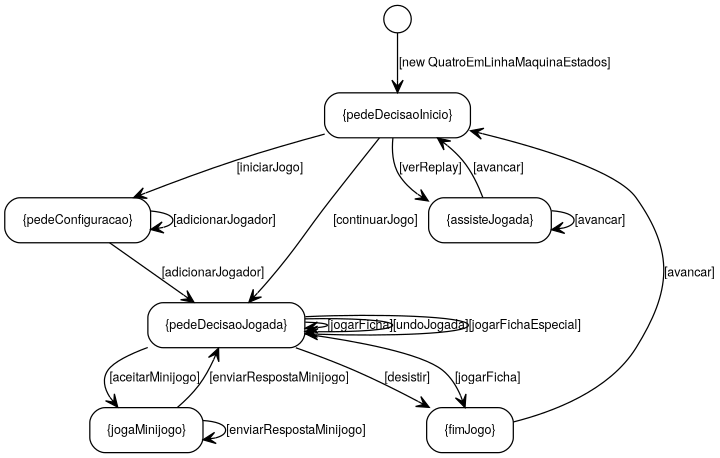
\includegraphics[width=0.8\textwidth]{diagrama-estados}
	 	\centering
	 	\caption{Diagrama de Estados}
	 	\label{fig:diag-estados}
	 \end{figure}
	
	\pagebreak
	
	\large
	\subsection{Command}
	\normalsize
	
	Com o objetivo de implementar a funcionalidade de undo e replay, foi usado o padrão Command, embora um pouco alterado, comparativamente ao leccionado nas aulas. Neste caso, o undo é entendido como um elemento do jogo, logo é implementado também como um Command, que se limita a chamar o método undo dos comandos anteriores. A escolha de ser usado o Command e não o Memento (ou qualquer outro padrão) baseou-se no facto de que o Command permite uma maior perceção das mudanças ao jogo e uma redução do custo de memória. Neste caso, não foram encontradas desvantagens ao uso do Command.
	
	O Command, nesta implementação, tem a dupla funcionalidade de suportar o undo de jogadas e o replay de jogos. No caso de se querer fazer undo a jogadas, é chamado o comando DesfazerJogadas, que desfaz um certo número dado de jogadas feitas.
	
	Associado ao CommandManager, há um histórico completo de comandos executados - que inclui comandos de undo e derrotas/vitórias de minijogos. Quando se chega ao fim de um jogo, é guardado este CommandManager num ficheiro (cujo nome depende da data e hora do sistema). Para visualizar um replay, basta carregar este CommandManager e ir executando, um a um, num tabuleiro vazio, os comandos do histórico completo. Simples e intuitivo, certo?
	
	Para além da informação específica a cada comando, todos eles incluem um toString com informação associada ao acontecimento em questão. Isto faz com que seja possível descrever ao utilizador, por texto, durante o replay, o que aconteceu no jogo, em vez de só mostrar visualmente.
	
	\large
	\subsection{Factory}
	\normalsize
	
	Foi também usado o padrão Factory. Este padrão abstrai a criação de certos objetos, simplificando o código onde for usado. Neste caso, foi utilizado em duas situações distintas: a criação de jogadores e a escolha dos minijogos. A sua implementação verifica-se na classe \textbf{JogadorFactory}, onde devolve o jogador criado mediante o valor da enum \textbf{TipoJogador} dado, assim como classe \textbf{MinijogoFactory}, que trata de devolver, alternadamente, o minijogo a ser jogado.
	
	\pagebreak
	
	\large
	\section{Classes}
	\normalsize
	
	Ao todo, foram usadas 33 classes, de entre as quais 3 são abstratas, 4 interfaces e 3 enums. Dessas, as mais relevantes são as seguintes: 
	
	\begin{itemize}
		\item Interface \textbf{Estado} - Representa, de forma abstrata, os estados possíveis da máquina de estados. É implementada pela classe \textbf{EstadoAdapter}, que por sua vez é extendida pelas classes \textbf{AssisteJogada}, \textbf{FimJogo}, \textbf{JogaMinijogo}, \textbf{PedeConfiguracao}, \textbf{PedeDecisaoInicio}, \textbf{PedeDecisaoJogada}. Cada estado está também definido na enum \textbf{Situacao};
		\item Interface \textbf{Minijogo} - Representa, de forma abstrata, os minijogos possíveis. É implementada pela classe MinijogoAdapter, que por sua vez é extendida pelas classes \textbf{Calculos} (jogo dos cálculos referido no enunciado) e \textbf{Palavras} (jogo das palavras);
		\item Interface \textbf{Jogador} - Representa, de forma abstrata, um jogador. É implementada pela classe \textbf{JogadorAdapter}, que é posteriormente extendida pela classe \textbf{Humano} (jogador humano) e \textbf{Computador} (jogador que joga de forma autónoma). Cada tipo de jogador está definido na enum \textbf{TipoJogador};
		\item Interface \textbf{Command} - Representa, de forma abstrata, um comando a executar, disponibilizando, também, caso seja necessário, o seu undo. É implementada pela classe \textbf{CommandAdapter}, que é extendida pelas classes \textbf{AdicionaFichaEspecial} (receber uma ficha especial devido a ter ganho um minijogo), \textbf{DesfazerJogadasCommand} (executa o undo de outros comandos), \textbf{DesistirCommand} (desistir do jogo), \textbf{JogarFichaCommand} (adicionar uma ficha numa coluna do tabuleiro), \textbf{JogarFichaEspecialCommand} e \textbf{PerderMinijogoCommand} (informação relativa à derrota num minijogo). Certas classes não têm undo possível, pois servem apenas para adicionar ao histórico completo de modo a possibilitar o replay;
		\item Classe \textbf{QuatroEmLinha} - Representa o jogo em si. Tem todos os métodos associados ao mesmo, como métodos para jogar uma ficha numa determinada coluna, ou adicionar um jogador. É constituída por dois objetos também essenciais à aplicação: um objeto da classe \textbf{Tabuleiro}, que trata de tudo o que tem a ver com a gestão do tabuleiro de jogo, e a classe \textbf{ListaJogador}, que gere a lista de jogadores a participar no jogo;
		\item Classe \textbf{CommandManager} - Recebe, executa e reverte comandos que lhe são enviados. Mantém um histórico destes comandos, servindo de base à implementação das funcionalidades de undo e replay;
		\item Classe \textbf{QuatroEmLinhaGestor} - Abstrai a interação com as classes \textbf{QuatroEmLinha} e \textbf{CommandManager}, controlando o que é executado diretamente e o que é executado através do Command;
		\item Classe \textbf{QuatroEmLinhaMaquinaEstados} - Serve de camada de interação entre as classes de IU e a classe \textbf{QuatroEmLinhaGestor}. É composta por um objeto do tipo \textbf{Estado}, e controla a interação com ele;
		\item Classe \textbf{QuatroEmLinhaMaquinaUITexto} - Classe que trata de toda a interação com o utilizador.
	\end{itemize}
	
	Embora já descrita acima, a relação entre as classes existentes é mais facilmente explicada pelo esquema presente na próxima página.
	
	\pagebreak
	
	Nota: As classes utilitárias e as enums não se encontram no esquema, devido a serem públicas e acessíveis em todo o programa.
	
	\vspace{0.5cm}
	
	\begin{figure}[h]
		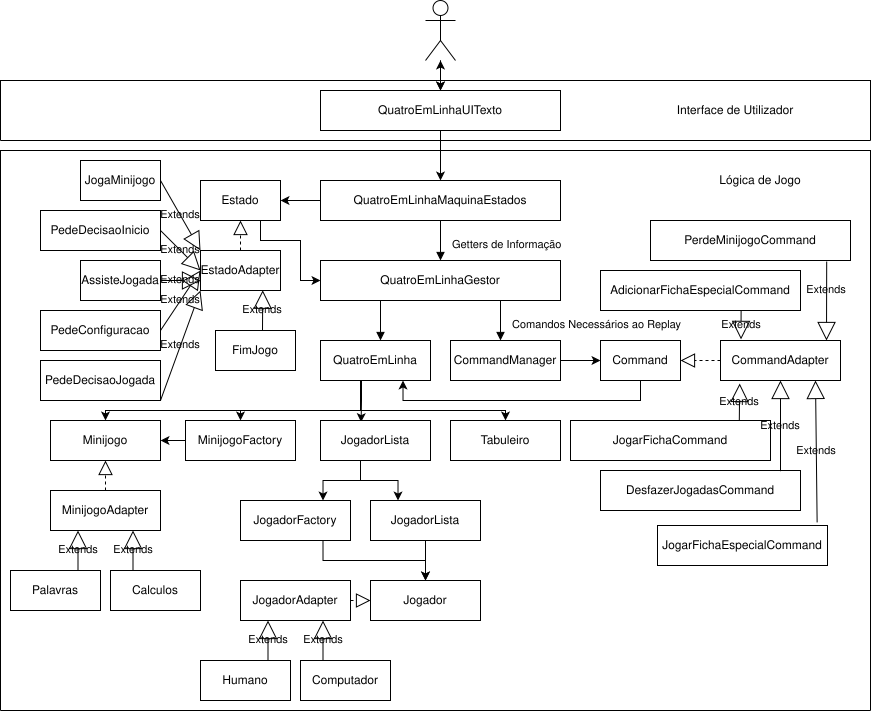
\includegraphics[width=1\textwidth]{diagrama-classes}
		\centering
		\caption{Diagrama de Classes}
		\label{fig:diag-classes}
	\end{figure}

	\pagebreak
	
	\large
	\section{Funcionalidades Implementadas}
	\normalsize
	\begin{center}
		\begin{tabular}{ |c|c|c|c| } 
			\hline
			\textbf{Componente do Trabalho} & \textbf{Realizado} & \textbf{Realizado parcialmente} & \textbf{Não realizado} \\ \hline
			Organização ficheiros / classes & \checkmark & & \\ \hline
			Nome e Tipo dos Jogadores & \checkmark & & \\ \hline
			Quatro em Linha Tradicional & \checkmark & & \\ \hline
			Minijogos e Peça Especial & \checkmark & & \\ \hline
			Replay dos 5 Últimos jogos & \checkmark & & \\ \hline
			Save e Load de Jogos a Decorrer & \checkmark & & \\ \hline
			Undos e Sistema de Créditos & \checkmark & & \\ \hline
		\end{tabular}
	\end{center}

	\large
	\section{Anexos}

	\normalsize
	\listoffigures
\end{document}